Una m\'aquina f\'abrica focos de 75 watts, donde el tiempo de vida \'util de los focos presenta un comportamiento de distribuci\'on
normal, donde el 16\% de los focos producidos duran menos de 1000.111 horas y el 12\% dura mas de 1043.5 horas
\begin{itemize}
	\item Calcule la media y varianza de la duraci\'on de los focos.\\
		$X~N(\mu,\sigma^{2})$\\
		Podemos desarrollar un sistema de ecuaciones, por cada porcentaje.\\
		Primero con($16\%$):\\
		$$P(X<1000.111)\ =\ 0.16$$
		$$P(Z<\frac{1000.111-\mu}{\sigma})\ =\ 0.16$$
		Mediante el comando \emph{qnorm(0.16)}, llegamos a:\\
		$$-0.99=\frac{1000.111-\mu}{\sigma}$$
		Por otro lado, con el otro porcentaje($12\%$):\\
		$$P(X>1043.5)\ =\ 0.12$$
		$$P(Z>\frac{1043.5-\mu}{\sigma})\ =\ 0.12$$
		Mediante la tabla:\\
		$$1.17=\frac{1043.5-\mu}{\sigma}$$
		Resolviendo el sistema de ecuaciones\\
		$$\sigma\ =\ 20.0875$$
		$$\mu\ =\ 1019.998$$
		$therefore\ Media=\mu=1019.988\ y\ Varianza=\mu^{2}=1040395.920 $\\
	\item ?`Cu\'al es la probabilidad de que un foco dure menos de 1000 horas?\\
		$P(X<1000)\ =\ 0.1597358\ $\\ %pnorm(1000,1019.998,20.0875)
	
	\item ?`Cu\'al es la probabilidad de que un foco dure m\'as de 1045 horas?\\
		Por simetr\'ia, es lo mismo que dure menos que 1045 horas\\
		$P(X>1045)\ =\ 1\ -\ P(X<1045)\ =\ 1\ -\  0.8933706\ =\ 0.1066294$\\ %pnorm(1000,1019.998,20.0875)
	\item ?` Que proporci\'on de focos duran entre 1000 y 1030 horas?\\
		% P(X<1030)-P(X<1000)
		% pnorm(1030,1019.998,20.0875)-pnorm(1000,1019.998,20.0875)
		$P(X<1030)-P(X<1000)\ =\ 0.5309946$\\
		
	\item Calcule $P(\mu - \sigma < X < \mu + \sigma)$, $P(\mu - 2\sigma < X < \mu + 2\sigma)$ y $P(\mu - 3\sigma < X < \mu + 3\sigma)$\\
		$P(999.9105 < X < 1040.086)\ =\ P(X<1040.086)-P(X<999.9105)\ =\ 0.6826955$\\
		$P(979.8230 < X < 1060.173)\ =\ P(X<1060.173)-P(X<979.8230)\ =\ 0.9544997$\\
		$P(959.7355 < X < 1080.261)\ =\ P(X<1080.261)-P(X<959.7355)\ =\ 0.9973003$\\

	\item Calcule las probabilidades anteriores usando la tabla y compare los resultados. (hint: estandarice).

	$P(X<1040.086)-P(X<999.9105)$\\
	$ = P(\frac{X-\mu}{\sigma} < \frac{1040.086-\mu}{\sigma}) - P(\frac{X-\mu}{\sigma} < \frac{999.9105-\mu}{\sigma})$\\
	$ = P(Z < 1) - P(Z < -1)$\\
	$ = 1 - P(Z > 1) - P(Z > 1)$\\
	$ = 1 - 2 P(Z > 1)$\\
	$ = 1 - 2 * 0.1587$\\
	$ = 0.6826$\\

        $P(X<1060.173)-P(X<979.8230)$\\
        $ = P(\frac{X-\mu}{\sigma} < \frac{1060.173-\mu}{\sigma}) - P(\frac{X-\mu}{\sigma} < \frac{979.8230-\mu}{\sigma})$\\
        $ = P(Z < 2) - P(Z < -2)$\\
	$ = 1 - P(Z > 2) - P(Z > 2)$\\
	$ = 1 - 2 P(Z > 2)$\\
	$ = 1 - 2 * 0.0228$\\
	$ = 0.9544$\\

        $P(X<1080.261)-P(X<959.7355)$\\
        $ = P(\frac{X-\mu}{\sigma} < \frac{1080.261-\mu}{\sigma}) - P(\frac{X-\mu}{\sigma} < \frac{959.7355-\mu}{\sigma})$\\
        $ = P(Z < 3) - P(Z < -3)$\\
	$ = 1 - P(Z > 3) - P(Z > 3)$\\
	$ = 1 - 2 P(Z > 3)$\\
	$ = 1 - 2 * 0.0013$\\
	$ = 0.9974$\\

	\item Realice gr\'aficos de la funci\'on de densidad de probabilidad y de la funci\'on de distribuci\'on.
	% x<-seq(900,1100,10)
	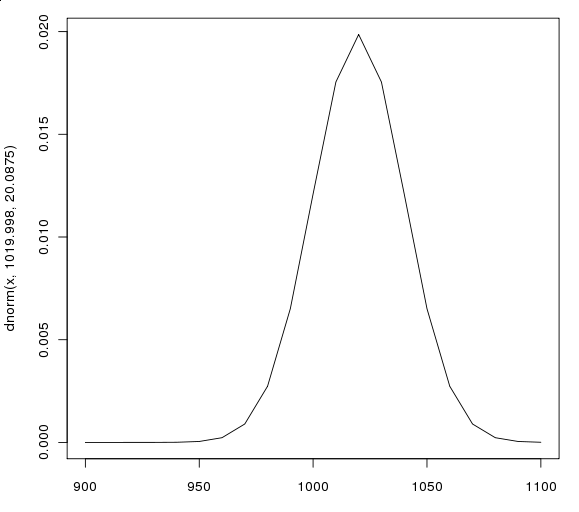
\includegraphics[scale=0.5]{images/2_2-dnorm}\\	% plot(x,dnorm(x,1019.998,20.0875),type="l") % Densidad
	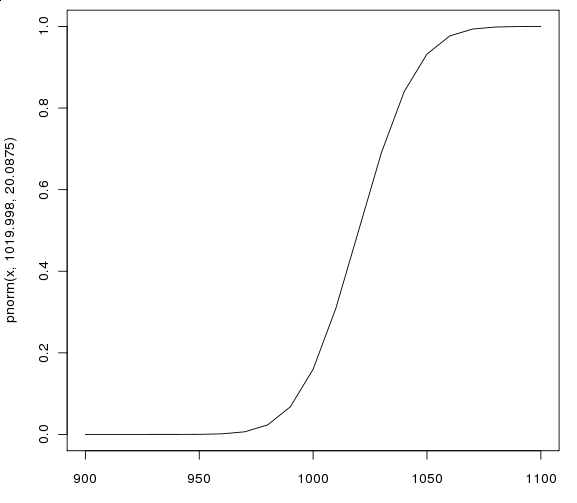
\includegraphics[scale=0.5]{images/2_2-pnorm}	% plot(x,pnorm(x,1019.998,20.0875),type="l") % Distribucion
	\item Var\'ie el o los valores de los par\'ametros de la distribuci\'on y comente lo observado en los gr\'aficos de la funci\'on de densidad y de distribuci\'on. (2 casos).

	\begin{itemize}
		\item Funcion de Densidad\\
	Variando Mu (900.998):\\
	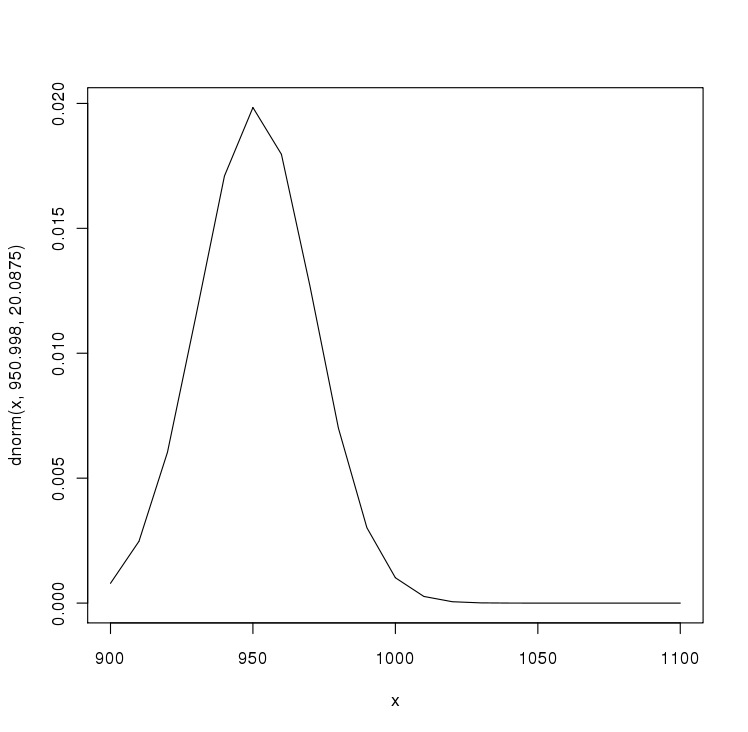
\includegraphics[scale=0.5]{images/2_2-dnorm-variado1}\\
	Variando Mu (1000.998):\\
	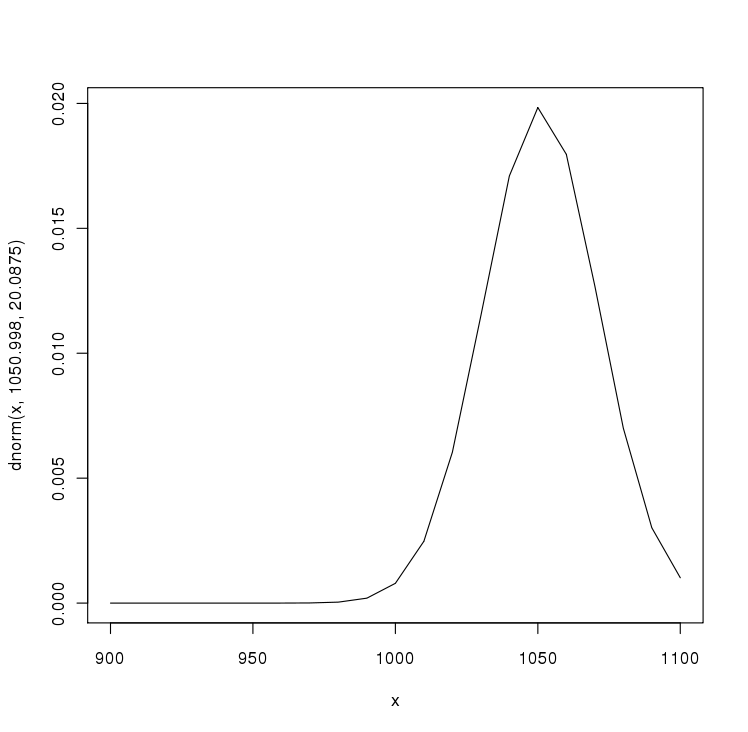
\includegraphics[scale=0.5]{images/2_2-dnorm-variado2}\\
	Como podemos observar, al variar Mu se refleja una traslaci\'on de la funci\'on.\\
		\item Funcion de Distribucion\\
	        Variando Mu (950.998):\\
        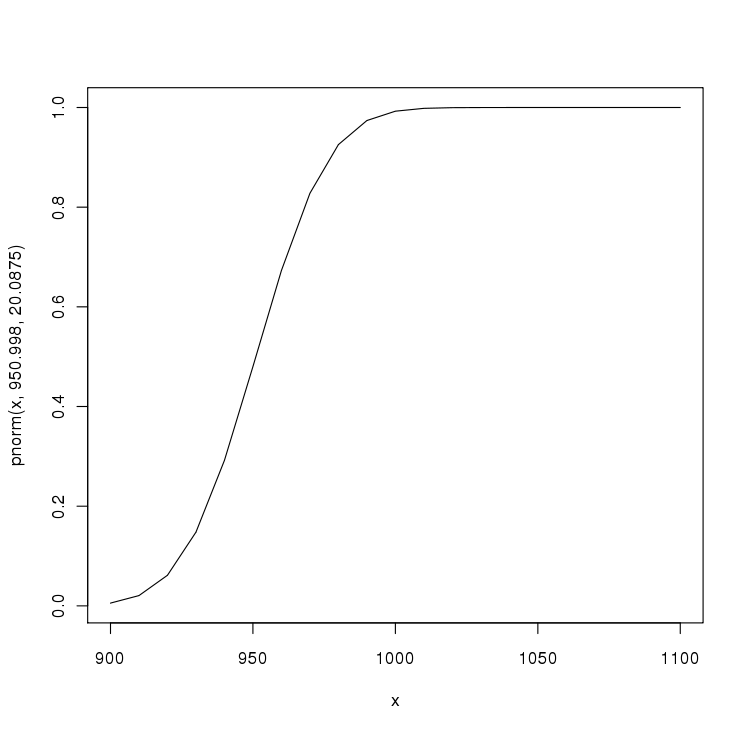
\includegraphics[scale=0.5]{images/2_2-pnorm-variado1}\\
        Variando Mu (1050.998):\\
        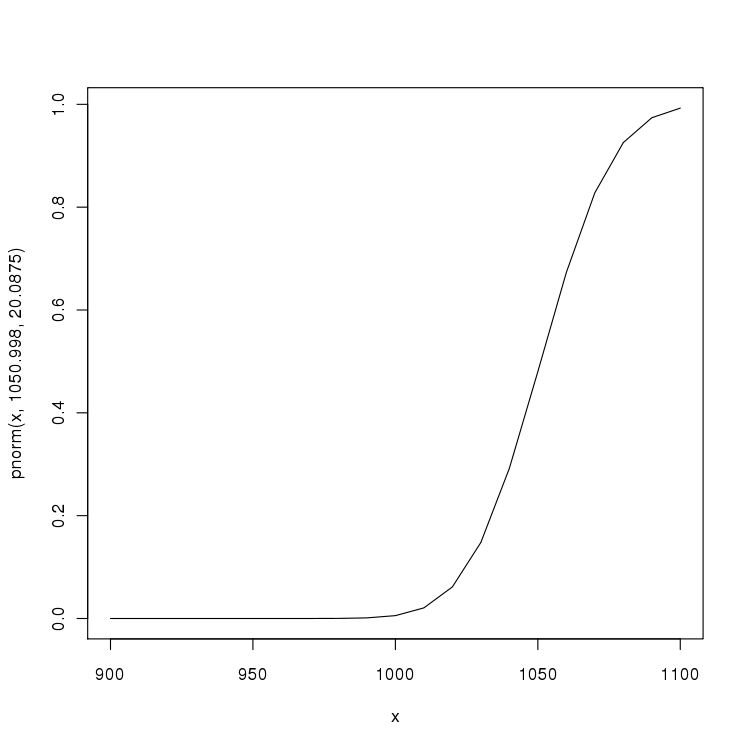
\includegraphics[scale=0.5]{images/2_2-pnorm-variado2}\\
        En la funcion de distribucion, si variamos Mu podemos ver que se desplaza el inicio de la funci\'on.\\
			
	\end{itemize}
\end{itemize}
